
\documentclass[runningheads, envcountsame, a4paper]{llncs}

% Recommended, but optional, packages for figures and better typesetting:
%\usepackage{microtype}
\usepackage{graphicx}
\usepackage{amsmath}
%\usepackage{amsthm}
\usepackage{amssymb}
%\usepackage{thmtools}
\usepackage{mathtools}	
\usepackage{pgfplots}
%\usepackage{hyperref}
%\usepackage{subcaption}
\usepackage[misc]{ifsym}

\DeclareMathOperator{\E}{\mathbb{E}}
\DeclareMathOperator{\p}{\mathbb{P}}
\pgfplotsset{
    colormap={blackwhite}{[5pt]
        rgb255(0pt)=(255, 255, 0);
        rgb255(85pt)=(0, 0, 0);
        rgb255(95pt)=(0, 0, 255);
        rgb255(500pt)=(200, 255, 255);
        rgb255(1000pt)=(200, 255, 255)
    },
}
%\renewcommand{\qedhere}{\begin{equation}\tag*{$\blacksquare$}\end{equation}}
%\newtheorem{Lemma}{Lemma}
%\newtheorem{Theorem}{Theorem}
%\newcommand{\theHalgorithm}{\arabic{algorithm}}




\begin{document}

\title{An Engineered Empirical Bernstein Bound\thanks{A great thanks to Sylvie Thi\'ebaux for advice and encouragement.}
}

\author{Mark A. Burgess\inst{1} (\Letter) \and
Archie C. Chapman\inst{2} \and
Paul Scott\inst{1}}

\authorrunning{M. Burgess, A. Chapman, P. Scott}
\institute{Australian National University, \\College of Engineering \& Computer Science, ACT, 0200, Australia. \\\email{markburgess1989@gmail.com, mark.burgess@anu.edu.au}\\\email{paul.scott@anu.edu.au}\vspace{2mm}\and
University of Sydney, \\School of Electrical and Information Engineering, NSW, 2006, Australia \\\email{archie.chapman@sydney.edu.au}}

\toctitle{An Engineered Empirical Bernstein Bound}
\tocauthor{M.~Burgess, A.~Chapman, P.~Scott}

\maketitle
\setcounter{footnote}{0}

\begin{abstract}
We derive a tightened \textit{empirical Bernstein bound} (EBB) on the variation of the sample mean from the population mean, and show that it improves the performance of \textit{upper confidence bound} (UCB) methods in multi-armed bandit problems.
Like other EBBs, our EBB is a concentration inequality for the variation of the sample mean in terms of the sample variance.
Its derivation uses a combination of probability unions and Chernoff bounds for the mean of samples and mean of sample squares.
Analysis reveals that our approach can tighten the best existing EBBs by about a third, 
and thereby halves the distance to a bound constructed with perfect variance information.
We illustrate the practical usefulness of our novel EBB by applying it to a multi-armed bandit problem as a component of a UCB method. 
Our method outperforms existing approaches by producing lower expected regret than variants of UCB employing several other bounds, including state-of-the-art EBBs.
\keywords{Concentration inequality \and Chernoff bounds \and Hoeffding's inequality \and Empirical Bernstein bound}
\end{abstract}


\section{Introduction}

Data-driven processes and decision-making applications typically rely on sample statistics 
to infer parameters of a population or evaluate decision options.
Depending on the domain, different assumptions can be made about the distribution of the data, 
which in turn determine which computational routines are used to compute the required population statistics. 
These assumptions may be based on prior information, expert opinion, or 
determined from the characteristics of the system under observation.

Within this context, finite-sample \textit{concentration inequalities} are used to place bounds on 
the variation of sample statistics around their population values.
Such bounds are applied in a range of data science contexts for a variety of prediction, machine learning and hypothesis testing tasks, including:
change detection \cite{KiferShaiGehrke2004,8000571} 
and classification \cite{Zia-UrRehman2012} in data streams;
outlier analysis in large databases \cite{Aggarwal2015};
online optimisation \cite{FlaxmanKalaiMcMahan2005,AgarwalDekelXiao2010}; and, of most relevance to this paper, 
online prediction and learning problems \cite{Cesa-BianchiLugosi2006,%Maron1997,
Mnih:2008:EBS:1390156.1390241,DBLP:conf/aaai/ThomasTG15,Maurer50empiricalbernstein},
particularly in settings with \textit{bandit feedback} \cite{AuerCesa-BianchiEtal_SIAM2003,AudibertBubeck_COLT2009,Tran-ThanhChapmanRJ_AAAI2009}. 
% Bandit feedback describes settings where a decision-maker wishes to learn about a system, and to do this, chooses samples from a set of actions and receives feedback regarding their chosen actions only, in the form of a realization of a random variable. 
%Specifically, the decision-maker does not see how the system would have responded, if they had chosen a different action.
%
In particular, the recently developed \textit{empirical Bernstein bounds} (EBB) are of significant interest ~\cite{Maurer50empiricalbernstein,10.1007/978-3-540-75225-7_15}. 
These are probability bounds describing the likely difference of a sample mean from the population mean 
in terms of the \textit{sample} variance, 
under the assumption that the population data is bounded within an interval of known width.
EBBs have been used as a method of generating confidence bounds for the mean, and an outstanding task is to see how much these techniques can be improved.

Given this challenge, in this work, we take inspiration and extend the work of  Maurer and Pontil (\cite{Maurer50empiricalbernstein}, M\&P in the remainder)
%combined with older techniques, 
to develop a new EBB.
Our EBB tightens existing bounds by incorporating a combination of bounds on the variation of the sample variance.
Specifically, we use two Chernoff bounds, for the sample mean and the mean of sample squares, which are fused using a probability union and variance decomposition,
to create a novel probability bound for the sample variance, which is then used to derive our novel EBB.

Evaluations show that our EBB significantly tightens the current state-of-the-art bounds. 
Specifically, our EBB can shrink the best existing EBBs by about a third. This represents half of the distance between the best existing EBBs and an unattainable Bernstein bound constructed with perfect variance information.
Moreover, we demonstrate the use of our novel EBB in an \textit{upper-confidence bound} (UCB) multi-armed bandit (MAB) algorithm.  
Results from a set of MABs show that using our bound in a UCB algorithm outperforms existing approaches, by producing comparable or lower expected regret than employing other existing bounds, including state-of-the-art EBBs.


The paper is organised as follows. 
Related work and preliminary concepts are reviewed in Sections~\ref{sec:related-work} and~\ref{sec:preliminaries}, respectively.
Our main results are in Section~\ref{derivation}, where we derive %a novel probability bound for the sample variance, and use this to create 
a novel EBB.
In Section~\ref{evaluation} we evaluate our EBB and show its improvements over existing bounds. 
In Section~\ref{sec:bandits} we apply it to a multi-armed bandit problem as part of a UCB algorithm, which demonstrates how our tighter EBB improves the algorithm's learning performance.
Section \ref{sec:conclusion} concludes.


\section{Related Work}\label{sec:related-work}
Concentration inequalities are probabilistic bounds describing how far a random variable is expected to deviate from (or otherwise be concentrated around) a particular value.
Most classic concentration inequalities describe the expected deviation of sample statistics, including 
Chebyshev's inequality~\cite{Chebyshev1}, 
the Bernstein's inequalities~\cite{Burnstein1}, 
Hoeffding's inequalities~\cite{hoeffding1} and 
Bennett's inequalities~\cite{10.2307/2282438}.
Building on these, new analysis has yielded a wide range concentration inequalities and methods of generating them ~\cite{MR3363542,Boucheron2004}. 
In particular, recent innovations concern the concentration of more-general functions of random variables, such as 
the Efron-Stein~\cite{efron1981} and 
entropy methods~\cite{Boucheron_concentrationinequalities}, and 
applications of Talagrand's concentration inequality~\cite{Talagrand1995}.
Inequalities such as these are used to describe the expected variability of sample statistics, such as the distance of a sample mean from the population mean.

Furthermore, additional sample statistics can be used to tighten such bounds, because these statistics provide extra distributional information that are incorporated as a factor into classical inequalities. 
EBBs \cite{Maurer50empiricalbernstein,10.1007/978-3-540-75225-7_15} are one example of this, where sample variance information is used to tighten a classical Bernstein bound.
However, it remains to be seen how far bounds derived by this approach can be tightened.

% In addition, concentration inequalities that describe sampling without replacement can give additional tightening over those that assume sampling with replacement. This refinement was first demonstrated in \cite{serfling1974} with a martingale argument.
% More recently, this result was improved with a reverse martingale argument and used to extend M\&P's EBB to the case of sampling without replacement \cite{bardenet2015}.
% Furthermore, if small sample sizes are assumed, then it may be possible to derive perfectly tight %ideal 
% concentration inequalities in some circumstances, and there do exist some computational methods to derive these perfect bounds more generally \cite{OUQ1,doi:10.1137/13094712X}.
% However, in this paper we focus on refining bounds in the case of sampling with replacement in the context of large numbers of samples.


\section{Preliminaries}\label{sec:preliminaries}

To begin, we state three lemmas which form the basis for our derivation (proofs in Appendix \ref{appendix:small}).
The first is an often used result related to union bounds:

\begin{lemma}[Probability Union]\label{prob_union}
For any random variables $a,b$ and $c$:
\[\p(a>c) \; \le \; \p(a>b) + \p(b>c)\]
\end{lemma}

This result is used to bound the probability relationship between two variables via knowledge of the probability relationship between them and a third variable.
%
The second definition relates the value of the sample mean and the value of sample squares to the sample variance. It is expanded here because we will later use these relationships to create bounds for the sample variance from bounds on the sample squares and sample mean.

\begin{lemma}[Variance Decomposition]\label{variance1}
For $n$ samples $x_i$, sample mean $\hat{\mu} = \frac{1}{n}\sum_ix_i$, sample variance $\hat{\sigma}^2=\frac{1}{n-1}\sum_i(x_i-\hat{\mu})^2$, and average of sample squares $\hat{\sigma}_0^2 = \frac{1}{n}\sum_ix_i^2$, the following relationship holds:
% \begin{align*}
% \quad\hat{\sigma}^2 
% &=\frac{1}{n-1}\sum_i\left(x_i-\frac{1}{n}\sum_jx_j \right)^2 
%  =\frac{1}{n-1}\left(\sum_ix_i^2-\frac{1}{n}\sum_{i,j}x_ix_j \right) % \\
% &= \frac{n}{n-1}\left(\hat{\sigma}_0^2-\hat{\mu}^2\right)
% \end{align*}
% which rearranging gives:
\[ 
\hat{\sigma}_0^2=\hat{\mu}^2+\frac{n-1}{n}\hat{\sigma}^2
\]
\end{lemma}



In order to derive our novel bound, we use the next lemma, which encapsulates a range of inequalities called \textit{Chernoff bounds} that give bounds on the mean of random variables:

\begin{lemma}[Chernoff Bound]\label{chernoff1}
If $\hat{\mu}$ is sample mean of $n$ independent and identically distributed samples of random variable $X$ then for any $s>0$ and $t$:
\[ \p(\hat{\mu}\ge t)\le\E\left[\exp(sX)\right]^n\exp(-snt) \]
\end{lemma}

The proof of this statement is straightforward and uses Markov's inequality and the i.i.d of the samples.
In the next section, we use these components to derive the bounds on the sample mean and the mean of sample squares, 
which we then use to create a new EBB.


\section{Derivation and numerical implementation}
\label{derivation}
In this section, we derive two Chernoff bounds, 
for the sample mean and the mean of sample squares, (Lemmas~\ref{sample_squares} and~\ref{variance2}, respectively). 
These are fused using a probability union and variance decomposition, defined above, to derive a bound for the sample variance. 
This bound is then used to derive our new EBB, as presented in Theorem~\ref{ebb1}.
However, due to its analytic intractability, we complete the derivation by discussing how to numerically implement the bound.

\subsection{Derivation}
Our first probability bound is a Chernoff bound on the sample mean called \textit{Bennett's inequality}. 
This bound is not new and was derived by \cite{hoeffding1} and \cite{10.2307/2282438} and has subsequently been a subject of discussion and many further developments \cite{Bentkus08boundsfor,Pinelis2014,zbMATH00812598}; we %give a statement of Bennett's inequality as lemma \ref{hoeffdings1} and also 
provide a proof in Appendix \ref{appendix:A}.

\begin{theorem}[Bennett's inequality]\label{hoeffdings1}
Let $X$ be a real-valued random variable with a mean of zero and variance $\sigma^2$, that is bounded $a\le X\le b$. 
Then for $t>0$, the mean $\hat{\mu}$ of $n$ samples of $X$ is probability bounded by:
\begin{equation}\label{eq_no2}\p(\hat{\mu}\ge t)\le H_1^n\left(\frac{\sigma^2}{b^2},\frac{t}{b}\right),
\end{equation}
where:
\begin{equation*}
H_1^n\left(\frac{\sigma^2}{b^2},\frac{t}{b}\right) =
\left(\left(\frac{\frac{\sigma^2}{b^2}}{\frac{\sigma^2}{b^2}+\frac{t}{b}}\right)^{\frac{\sigma^2}{b^2}+\frac{t}{b}}
\left(1-\frac{t}{b}\right)^{\frac{t}{b}-1}\right)^{\frac{n}{\frac{\sigma^2}{b^2}+1}}
\end{equation*}
\end{theorem}

We will also use a double-sided version of this bound:
\begin{equation}\label{eq_no1}\p(\hat{\mu}^2\ge r^2) \le H_1^n\left(\frac{\sigma^2}{b^2},\frac{r}{b}\right) + H_1^n\left(\frac{\sigma^2}{a^2},\frac{-r}{a}\right) \end{equation}

The assumption that the mean is zero can be used without a loss of generality.
In this way, Bennett's inequality gives us a probability bound for the difference of the sample mean from the true mean \textit{given the variance}.

However, often in practice the variance is unknown, 
but can only estimate it via a sample variance statistic.
Thus, we derive a bound the difference of the sample variance from the variance as follows (proof in Appendix \ref{appendix:B}):

\begin{lemma}[Sample square bound]\label{sample_squares}
Let $X$ be a real-valued random variable with a mean of zero and variance $\sigma^2$, that is bounded $a\le X\le b$, if $d=\max(b,-a)$ then for $y>0$, the mean of sample squares $\hat{\sigma}_0^2=\frac{1}{n}\sum_ix_i^2$ is probability bounded:
\begin{equation}\label{equation_squares}\p(\sigma^2 - \hat{\sigma}_0^2> y) \le H_2^n\left(\frac{\sigma^2}{d^2},\frac{y}{d^2}\right),
\end{equation}
where:
\begin{align*} H_2^n\left(\frac{\sigma^2}{d^2},\frac{y}{d^2}\right) = \left(
\left(\frac{1-\frac{\sigma^2}{d^2}}{1+\frac{y}{d^2}-\frac{\sigma^2}{d^2}}\right)^{1+\frac{y}{d^2}-\frac{\sigma^2}{d^2}}
\left(\frac{\frac{\sigma^2}{d^2}}{\frac{\sigma^2}{d^2}-\frac{y}{d^2}}\right)^{\frac{\sigma^2}{d^2}-\frac{y}{d^2}}
\right)^n
\end{align*}
\end{lemma}


It is worth noting that we choose to restrict the use of function $H_2^n$ to cases which are sensible for it to be applied:
(i) it is defined for $a<0<b$, because otherwise the mean could not be zero), and (ii) $\sigma^2\le-ab\le (b-a)^2/4$ by Popoviciu's inequality \cite{zbMATH05780164}, as it is not possible for the variance to be larger given the width of the data bounds.  
It is important that these domain restrictions are conserved with the analysis.

At this point, we have a probability bound on the mean squared (Equation \ref{eq_no1}) 
and a probability bound on the sample squares (Lemma \ref{sample_squares}). With these in hand, we use lemma \ref{variance1} to create a bound on the sample variance, as follows.

\begin{lemma}[Sample Variance Bound]\label{variance2}
For a random variable that is bounded $a\le X\le b$ with variance $\sigma^2$ and a mean of zero, if $d=\max(b,-a)$ then for $w>0$, the sample variance $\hat{\sigma}^2$ of $n$ samples is probability bounded by:
\begin{equation}\label{eq_no8}
\p(\sigma^2 - \hat{\sigma}^2 > w) \le H_3^n(a,b,w,\sigma^2),
\end{equation}
where:
\begin{align*} H_3^n(a,b,w,\sigma^2) =\min_{\phi\in[0,1]}
\begin{Bmatrix}
	H_1^n\left(\frac{\sigma^2}{b^2},\frac{\sqrt{\phi(\frac{n-1}{n}w+\frac{1}{n}\sigma^2)}}{b}\right)\\
	+H_1^n\left(\frac{\sigma^2}{a^2},\frac{-\sqrt{\phi(\frac{n-1}{n}w+\frac{1}{n}\sigma^2)}}{a}\right)\\
	+H_2^n\left(\frac{\sigma^2}{d^2},\frac{(1-\phi)(\frac{n-1}{n}w+\frac{1}{n}\sigma^2)}{d^2}\right)
\end{Bmatrix}\end{align*}
\end{lemma}

A proof is provided in Appendix \ref{appendix:B}.
The use of the function $H_3^n$ is subject to the same restrictions on its domain as $H_2^n$.
Thus, in Lemma \ref{hoeffdings1} we have a bound for the sample mean given the variance, and in Lemma \ref{variance2} we have a probability bound for the difference of the sample variance from the population variance. 
Next, we outline a method of combining these two to create a bound for the sample mean given the sample variance --- and thereby derive a new empirical Bernstein bound.
To do this, we now expound a theorem that embodies a process %slightly improved
followed by M\&P \cite{Maurer50empiricalbernstein}. 

Before beginning, we introduce some notation.
For a function $f$ with ordered inputs, 
we denote the inverse of $f$ with respect to its $i${th} input 
(counting from one) as $f^{-(i)}$, assuming it exists.
Denote probability bounds on the differences of the sample mean from the mean, and the sample variance from the variance, by
$\p(\hat{\mu}-\mu>t)\le h(\sigma^2,t)$ and $\p(\sigma^2-\hat{\sigma}^2>w)\le f(\sigma^2,w)$, respectively.
Note that functions $h$ and $f$ have arguments $\sigma^2$ and $t$, and $\sigma^2$ and $w$, respectively.

\newpage

\begin{theorem}[Essential EBB]\label{ebb1} 
Assume $f^{-(2)}$ and $h^{-(2)}$ both exist, and also if $h^{-(2)}$ is monotonically increasing in its first argument, so that we can define:
\[
z(\sigma^2,w) = \sigma^2-f^{-(2)}\left(\sigma^2,w\right)
\]
If $z^{-(1)}$ exists and is monotonic increasing in its first argument, then for any $x\in[0,y]$, the following relationship holds:
\[
\p\left(\hat{\mu}-\mu>h^{-(2)}\left(z^{-(1)}\left(\hat{\sigma}^2,y-x\right),x\right)\right)
\le y
\]
\end{theorem}
%
\begin{proof}
Substituting $w$ for $f^{-2}(\sigma^2,w)$ gives:
%$\p(\sigma^2-\hat{\sigma}^2>f^{-2}(\sigma^2,w))\le w$\\
%$\p(z(\sigma^2,w)>\hat{\sigma}^2)\le w$\\
%$\p(\sigma^2>z^{-1}(\hat{\sigma}^2,w))\le w$\\
%$\p(h^{-2}(\sigma^2,t)>h^{-2}(z^{-1}(\hat{\sigma}^2,w),t))\le w$\\
\begin{align*}
w & \ge \p\left(\sigma^2-\hat{\sigma}^2>f^{-(2)}\left(\sigma^2,w\right)\right)\\
 & \ge \p\left(z\left(\sigma^2,w\right)>\hat{\sigma}^2\right)\\
 & \ge \p\left(\sigma^2>z^{-(1)}\left(\hat{\sigma}^2,w\right)\right)\\
 & \ge \p\left(h^{-2}\left(\sigma^2,t\right)>h^{-(2)}\left(z^{-(1)}\left(\hat{\sigma}^2,w\right),t\right)\right)
\end{align*}
% $w  \ge \p(\sigma^2-\hat{\sigma}^2>f^{-2}(\sigma^2,w))$\\
% \-\hspace{4mm}$\ge \p(z(\sigma^2,w)>\hat{\sigma}^2)$\\
% \-\hspace{4mm}$\ge \p(\sigma^2>z^{-1}(\hat{\sigma}^2,w))$\\
% \-\hspace{4mm}$\ge \p(h^{-2}(\sigma^2,t)>h^{-2}(z^{-1}(\hat{\sigma}^2,w),t))$\\
Substituting $t$ for $h^{-(2)}(\sigma^2,t)$ gives:
\[
\p\left(\hat{\mu}-\mu>h^{-(2)}\left(\sigma^2,t\right)\right)
\le t.
\]
Applying probability union (lemma \ref{prob_union}) gives:\\
\[
\p\left(\hat{\mu}-\mu>h^{-(2)}\left(z^{-(1)}\left(\hat{\sigma}^2,w\right),t\right)\right)
\le t+w.
\]
Letting $y=t+w$ and $x=y-w$ completes the proof.$\hfill\blacksquare$
\end{proof}

The result of this Theorem is an EBB, and our novel EBB is completed by substituting  $h(\sigma^2,t)=H_1^n\left(\sigma^2/b^2,t/b\right)$ and $f(\sigma^2,w)=H_3^n\left(a,b,w,\sigma^2\right)$ into Theorem \ref{ebb1}. 
Care must be taken in applying this theorem that all the assumptions hold, 
the inverses exist, and the domains of the functions are propagated through the analysis.




\subsection{Numerical Implementation}
\label{numerical-implementation}
Analytically solving this new EBB is challenging, however it is possible to evaluate it to arbitrary accuracy using numerical techniques.
This section provides a high-level description of a process for calculating our EBB.\footnote{sourcecode available at:\\\url{https://github.com/Markopolo141/Engineered-Empirical-Bernstein-Bound}}

This calculation is composed of three primary parts:
(i) the computation of function $f(\sigma^2,w)=H_3^n(a,b,y,\sigma^2)$;
(ii) verifying that the assumptions of Theorem \ref{ebb1} hold for $h(\sigma^2,t)=H_1$ and $f(\sigma^2,w)=H_3$, and;
(iii) calculating the subsequent result of Theorem \ref{ebb1}.

First, the function $f(\sigma^2,w)=H_3^n(a,b,w,\sigma^2)$ is the solution to an optimization problem that solves for the minima of an objective function subject to constraint $\phi\in[0,1]$.
Despite its complexity, a solution can be found quickly using a single variable parameter sweep.

Second, it is necessary to verify the assumptions that $h^{-(2)}$, $f^{-(2)}$ and $z^{-(1)}$ exist and that $z^{-(1)}$ and $f^{-(2)}$ are monotonically increasing in their first argument.
It is easy to note that $h(\sigma^2,t)=H_1^n\left(\sigma^2/b^2,t/b\right)$ is a closed-form function that is monotonically decreasing from $1$ to $0$ on the second argument, so $h^{-(2)}$ exists and is monotonically increasing in its first argument.  However the remaining assumptions are more difficult to verify.
For any function, the values that the function takes can be plotted as an array of points and the values that the inverse of that function takes can be determined by conducting coordinate swaps on those points.
The values of $f(\sigma^2,w)=H_3^n(a,b,w,\sigma^2)$ were computed and were seen to be monotonically decreasing in its second argument confirming that $f^{-(2)}$ exists.
The function $z(\sigma^2,w)=\sigma^2-f^{-(2)}\left(\sigma^2,w\right)$ is then seen to be a manipulation on the coordinate swapped points of $f(\sigma^2,w)=H_3^n(a,b,w,\sigma^2)$.
By coordinate swapping again, $z^{-(1)}$ was seen to be a regular function monotonically increasing on its first argument, hence satisfying assumptions.


Third, to numerically calculate the result of Theorem \ref{ebb1} the functions $h^{-(2)}$ and $z^{-(1)}$ were numerically evaluated by direct parameter searches and then composed as:
$h^{-(2)}(z^{-(1)}(\hat{\sigma}^2,y-x),x)$ - which is the inner part of the expression of the new EBB parameterised by $x$ explicitly and also $a,b$ implicitly.
%
However we typically don't know the values of $a$ and $b$, but instead know the mean is somewhere within a finite interval of width $D=b-a$.
Given this, we then take the worst case values of $a$ and $b$ consistent with a given $D$, 
and then take the best $x\in[0,y]$ subject to all other bounds.


\section{Comparison to existing bounds}\label{evaluation}
In this section, we make three comparisons of our results to existing concentration bounds, namely (i) Lemma \ref{variance2} is compared to M\&P's entropic bound, then 
our EBB is compared to (ii) M\&P's EBB and (iii) Bennett's inequality with perfect variance information.

First, M\&P's entropic bound \cite{Maurer50empiricalbernstein} 
(originally presented in \cite{MR2245497}) 
is given by:
\begin{equation}\label{eq:fe} 
\p(\sigma^2 - \hat{\sigma}^2>w) \le \exp\left(\frac{-(n-1)w^2}{2\sigma^2D^2}\right) 
\end{equation}
%
The improvement our variance bound (Lemma \ref{variance2}) offers over theirs is given by:
\begin{align}
Y\left(\frac{\sigma^2}{D^2},\frac{w}{D^2},n\right)
 =\exp\left(\frac{-(n-1)w^2}{2\sigma^2D^2}\right) -\max_{b} H_3^n\left(D(1-b),Db,w,\sigma^2\right)\label{eq:advantage}
\end{align}
where $b$ has a viable range between $0.5$ and $0.5-\sqrt{0.25-\sigma^2/D^2}$ (via Popoviciu's inequality).
Figure \ref{biggraph2} plots this improvement against $\sigma^2$ and $w$ for $n=200$, which shows large regions of advantage.
However, it is possible to use the minima of several different variance bounds, so in constructing our EBB, we take the minima of our variance bound and the entropic bound.

Second, we compare our EBB directly with M\&P's EBB~\cite{Maurer50empiricalbernstein}, 
given by:
\begin{equation}\label{maurersbound} \p\left(\mu-\hat{\mu}>\sqrt{\frac{2\hat{\sigma}^2\log(2/y)}{n}}+\frac{7D\log(2/y)}{3(n-1)}\right)<y. \end{equation}
In order to fairly compare our EBB to M\&P's we apply Popoviciu's inequality as a domain restriction, 
and carry it through their derivation, as we did to our own EBB. 
Specifically, this is the domain where:
\[ \frac{1}{2}>\frac{\sqrt{\hat{\sigma}^2}}{D}+\sqrt{\frac{2\log(2/y)}{n-1}} \]
We plot the improvement our EBB offers in this domain, as shown in Figure \ref{biggraph3}. 
In this plot, a probability 0.5 bound is shown to shrink by approximately one third.
More generally, we observe that our refinement of M\&P's EBB is be uniformly tighter across a large range of values.


\begin{figure}[t!]
\centering
\begin{tikzpicture}[scale=0.8]
	\begin{axis}[
	xmin=0,   xmax=0.25,
	ymin=0,   ymax=0.25,
	zmin=-0.15,   zmax=1.0,
	xtick={0.05,0.10,0.15,0.20,0.25},
	ytick={0.05,0.10,0.15,0.20},
	%ztick={-0.2,-0.1,0,0.1},
	xlabel=$\frac{\sigma^2}{D^2}$,
	ylabel=$\frac{w}{D^2}$,
	%zlabel=$blah$,
	xticklabel style={/pgf/number format/fixed},
	yticklabel style={/pgf/number format/fixed},
	zticklabel style={/pgf/number format/fixed},
	view={-105}{35},
	%point meta min=-0.3, point meta max=0.3,
	point meta min=-0.1, point meta max=1.0,
	title={Advantage over Entropic bound for n=200},
	%colorbar horizontal,
	colorbar,
	colorbar style={
		at={(1.07,0.64)},
		%title=Advantage,
		%ylabel=Z-value,
		%ytick={-1,-0.75,...,1},
		height=0.52*\pgfkeysvalueof{/pgfplots/parent axis height},
		xticklabel style={
			text width=2.5em,
			%align=below,
			%anchor=north west,
			/pgf/number format/.cd,
			fixed,
			fixed zerofill
		}
	}
	]
	\addplot3[patch, shader=flat] 
	file
	{graph1.dat};
	\end{axis}
\end{tikzpicture}
	\vspace{-5pt}
\caption{The strength of our variance bound over Maurer's Entropic bound. The graph of $Y\left(\frac{\sigma^2}{D^2},\frac{w}{D^2},n\right)$ from Equation \ref{eq:advantage}}\label{biggraph2}
\end{figure}


\begin{figure}[]{}
    \centering
	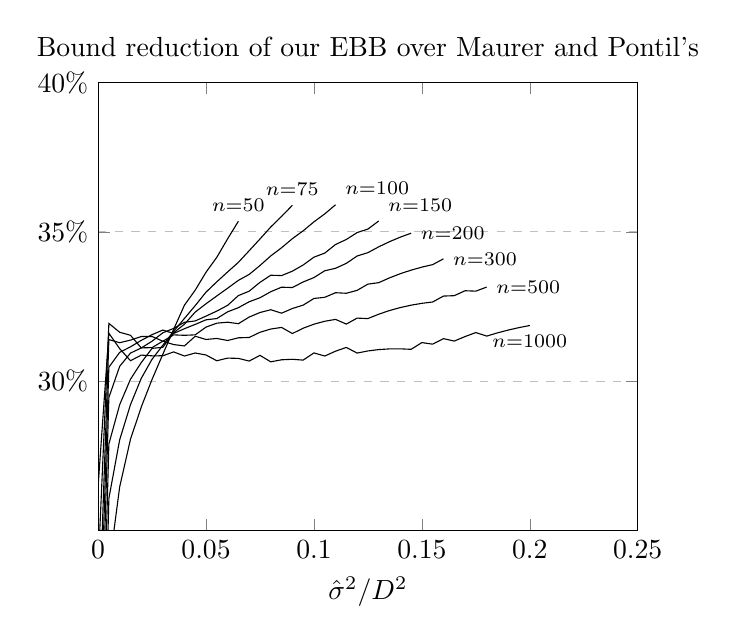
\begin{tikzpicture}
	\begin{axis}[
		title={Bound reduction of our EBB over  Maurer and Pontil’s},
		xlabel={$\hat{\sigma}^2/D^2$},
		xmin=0, xmax=0.25,
		ymin=25, ymax=40,
		xtick={0,0.05,0.1,0.15,0.2,0.25},
		ytick={30,35,40},
		yticklabel=$\pgfmathprintnumber{\tick}\%$,
		ymajorgrids=true,
		grid style=dashed,
		xticklabel style={/pgf/number format/fixed},
	]
	\addplot[] coordinates {
(0.0, 10.038489469957923)(0.005, 23.729228874038338)(0.01, 26.46795119155083)(0.015, 28.061119743643296)(0.02, 29.141938583623652)(0.025, 30.066155991693723)(0.03, 30.907282335052788)(0.035, 31.738722848538305)(0.04, 32.54914392836502)(0.045, 33.05291848928947)(0.05, 33.651509619741496)(0.055, 34.151805087746446)(0.06, 34.768247610158575)(0.065, 35.35764746719292)
		}node[pos=1.0](endofplotsquare){} ;
	\node [above] at (endofplotsquare) {$\scriptstyle n=50$};
	\addplot[] coordinates {
(0.0, 12.591458904845746)(0.005, 26.08582516018055)(0.01, 28.044488963240152)(0.015, 29.219014176778845)(0.02, 30.101019545112305)(0.025, 30.739739304373572)(0.03, 31.209391146592484)(0.035, 31.67459564986504)(0.04, 32.10560417423678)(0.045, 32.53522214247566)(0.05, 32.98480753922602)(0.055, 33.33123349968554)(0.06, 33.66064263107598)(0.065, 33.983296057116895)(0.07, 34.371432119724126)(0.075, 34.76400092304011)(0.08, 35.165771922230526)(0.085, 35.51929445366766)(0.09, 35.890640326573575)
		}node[pos=1.0](endofplotsquare){} ;
	\node [above] at (endofplotsquare) {$\scriptstyle n=75$};
	\addplot[] coordinates {
(0.0, 14.817995440815901)(0.005, 27.90751007185735)(0.01, 29.219819451516923)(0.015, 30.070639062533996)(0.02, 30.629290720122317)(0.025, 31.104197838170627)(0.03, 31.14038996461402)(0.035, 31.62526607199946)(0.04, 31.911575841232846)(0.045, 32.3187069670152)(0.05, 32.59698646227685)(0.055, 32.85814963311234)(0.06, 33.115830685662)(0.065, 33.379908028841236)(0.07, 33.578110917203176)(0.075, 33.87653264786374)(0.08, 34.19803078792182)(0.085, 34.470564003329045)(0.09, 34.774201537103245)(0.095, 35.03784322660741)(0.1, 35.337583634279)(0.105, 35.60362789769355)(0.11, 35.90890662248758)
		}node[pos=1.0](endofplotsquare){} ;
	\node [above right] at (endofplotsquare) {$\scriptstyle n=100$};
	\addplot[] coordinates {
(0.0, 17.342661445161745)(0.005, 29.461247776997926)(0.01, 30.502124709956824)(0.015, 30.94634600450878)(0.02, 31.116833768989828)(0.025, 31.344627574353588)(0.03, 31.62499327739429)(0.035, 31.772139980592)(0.04, 31.975727165299386)(0.045, 32.02196228998142)(0.05, 32.183034431467235)(0.055, 32.352369659168474)(0.06, 32.54250416890406)(0.065, 32.87047963677422)(0.07, 33.017679271803296)(0.075, 33.31333732160584)(0.08, 33.55087101615144)(0.085, 33.53938459819124)(0.09, 33.68714872653657)(0.095, 33.89275583281304)(0.1, 34.15600891069251)(0.105, 34.290920495879966)(0.11, 34.57974857223946)(0.115, 34.747357884723435)(0.12, 34.97811379083637)(0.125, 35.09584827017029)(0.13, 35.36531839253051)
		}node[pos=1.0](endofplotsquare){} ;
	\node [above right] at (endofplotsquare) {$\scriptstyle n=150$};
	\addplot[] coordinates {
(0.0, 19.269181617386778)(0.005, 30.47328215171227)(0.01, 30.970505248952783)(0.015, 31.155076903228505)(0.02, 31.370737591330126)(0.025, 31.563153411429678)(0.03, 31.716924278688328)(0.035, 31.602163041853583)(0.04, 31.762160711176872)(0.045, 31.905759719654245)(0.05, 32.05956774531062)(0.055, 32.101874254626836)(0.06, 32.32639539364612)(0.065, 32.465858041087344)(0.07, 32.663895247621326)(0.075, 32.797586647322234)(0.08, 32.99998541625402)(0.085, 33.15092115439265)(0.09, 33.13907818080335)(0.095, 33.32527974281349)(0.1, 33.47347491095124)(0.105, 33.70030345616673)(0.11, 33.78337094262078)(0.115, 33.94866206353597)(0.12, 34.19406008169977)(0.125, 34.30666804274627)(0.13, 34.5014054670121)(0.135, 34.67351335871075)(0.14, 34.82497129829329)(0.145, 34.95753413863828)
		}node[pos=1.0](endofplotsquare){} ;
	\node [right] at (endofplotsquare) {$\scriptstyle n=200$};
	\addplot[] coordinates {
(0.0, 21.01455983414305)(0.005, 31.398323351742654)(0.01, 31.29316800287044)(0.015, 31.380044700971307)(0.02, 31.499573558604126)(0.025, 31.501955199548522)(0.03, 31.342388805161228)(0.035, 31.555898653589576)(0.04, 31.540720961712708)(0.045, 31.556719994430246)(0.05, 31.815518124296712)(0.055, 31.947447662218103)(0.06, 31.979020008525413)(0.065, 31.929950573976118)(0.07, 32.151946530365926)(0.075, 32.30372613153442)(0.08, 32.39631985663968)(0.085, 32.28147349936643)(0.09, 32.43775937546441)(0.095, 32.55064623256504)(0.1, 32.77372870056995)(0.105, 32.81284419609248)(0.11, 32.96572615770543)(0.115, 32.94748952790814)(0.12, 33.04474761150041)(0.125, 33.25359991684834)(0.13, 33.30204392434083)(0.135, 33.462830030160355)(0.14, 33.601886363972085)(0.145, 33.7211101175424)(0.15, 33.822185822075845)(0.155, 33.90661477833436)(0.16, 34.09961256888578)
		}node[pos=1.0](endofplotsquare){} ;
	\node [right] at (endofplotsquare) {$\scriptstyle n=300$};
	\addplot[] coordinates {
(0.0, 23.733576061543907)(0.005, 31.93999128292596)(0.01, 31.642400396531094)(0.015, 31.54212092349261)(0.02, 31.12052542652318)(0.025, 31.129819611252405)(0.03, 31.344098301521242)(0.035, 31.231838999520004)(0.04, 31.185453514912005)(0.045, 31.51029078782499)(0.05, 31.401697787018254)(0.055, 31.43592520457107)(0.06, 31.367624957687056)(0.065, 31.45753767654653)(0.07, 31.468778394474676)(0.075, 31.6423499409508)(0.08, 31.751037287923307)(0.085, 31.804794091938522)(0.09, 31.59991862434968)(0.095, 31.778311022724473)(0.1, 31.913384999263183)(0.105, 32.010501900631745)(0.11, 32.074189915872516)(0.115, 31.915973789453584)(0.12, 32.11613625130849)(0.125, 32.10053700848796)(0.13, 32.24708311545571)(0.135, 32.3692691037866)(0.14, 32.46936498795406)(0.145, 32.54937215145163)(0.15, 32.61106237732128)(0.155, 32.65601018366708)(0.16, 32.85390573088976)(0.165, 32.867317678660584)(0.17, 33.03199624865481)(0.175, 33.01872182909822)(0.18, 33.15487119563348)
		}node[pos=1.0](endofplotsquare){} ;
	\node [right] at (endofplotsquare) {$\scriptstyle n=500$};
	\addplot[] coordinates {
(0.0, 26.48466951022569)(0.005, 31.610541001763814)(0.01, 31.094245131329373)(0.015, 30.691021818068354)(0.02, 30.878933354114203)(0.025, 30.854623560301786)(0.03, 30.855718952687877)(0.035, 30.985476785778605)(0.04, 30.84839664811395)(0.045, 30.94907807084863)(0.05, 30.882232292715344)(0.055, 30.68950445827823)(0.06, 30.77857995587979)(0.065, 30.768677505684852)(0.07, 30.679146150855704)(0.075, 30.870441770906094)(0.08, 30.653781659199446)(0.085, 30.72198559607093)(0.09, 30.738566645167236)(0.095, 30.710992728150178)(0.1, 30.95229310334558)(0.105, 30.847606478652455)(0.11, 31.009527688997892)(0.115, 31.135832380489546)(0.12, 30.946326663430018)(0.125, 31.017664917855072)(0.13, 31.06348584444511)(0.135, 31.08638415275851)(0.14, 31.0886271157673)(0.145, 31.072204850949028)(0.15, 31.29715291414822)(0.155, 31.244828197450204)(0.16, 31.429852460842593)(0.165, 31.347766957340134)(0.17, 31.49894525891586)(0.175, 31.63356906325342)(0.18, 31.514234978296805)(0.185, 31.62214364046394)(0.19, 31.716729481001114)(0.195, 31.79891328121711)(0.2, 31.869534804168858)
		}node[pos=1.0](endofplotsquare){} ;
	\node [below] at (endofplotsquare) {$\scriptstyle n=1000$};
	\end{axis}
	\end{tikzpicture}
	\vspace{-10pt}
	\caption{The percent reduction of the 0.5 probability bound, that going from Maurer and Pontil's EBB to our EBB would achieve, for various $n$, in the domain valid for their EBB.}
	\label{biggraph3}
	
	
	\vspace{15pt}
	
	
	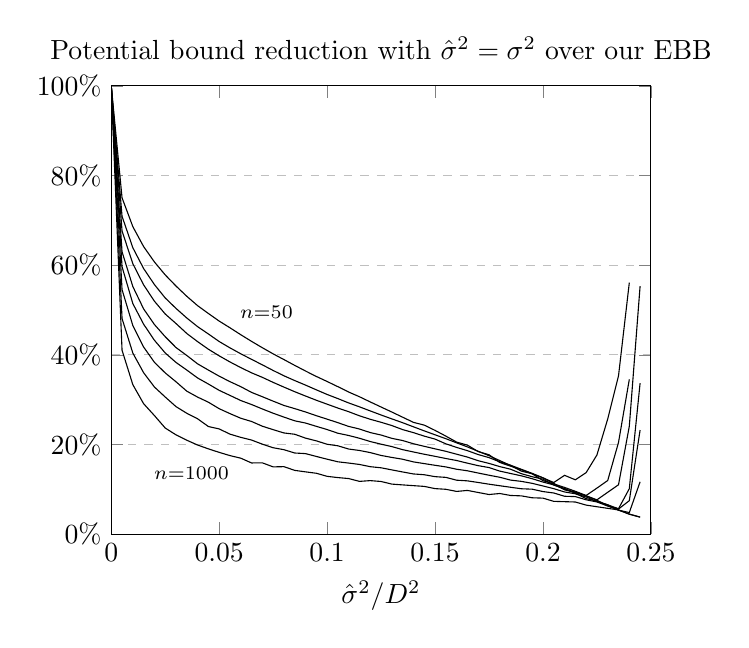
\begin{tikzpicture}
	\begin{axis}[
		title={Potential bound reduction with $\hat{\sigma}^2 = \sigma^2$ over our EBB},
		xlabel={$\hat{\sigma}^2/D^2$},
		xmin=0, xmax=0.25,
		ymin=0, ymax=100,
		xtick={0,0.05,0.1,0.15,0.2,0.25},
		ytick={0,20,40,60,80,100},
		yticklabel=$\pgfmathprintnumber{\tick}\%$,
		legend pos=south west,
		ymajorgrids=true,
		grid style=dashed,
		xticklabel style={/pgf/number format/fixed},
	]
	\addplot[] coordinates {
(0.0, 100.0)(0.005, 75.02420135527589)(0.01, 68.58202038924931)(0.015, 64.13237924865832)(0.02, 60.71118820468343)(0.025, 57.819103972950124)(0.03, 55.33498759305211)(0.035, 53.04630381803412)(0.04, 50.96)(0.045, 49.21383647798742)(0.05, 47.51937984496124)(0.055, 46.02446483180428)(0.06, 44.47806354009077)(0.065, 42.99625468164794)(0.07, 41.57386785449146)(0.075, 40.20618556701031)(0.08, 38.93352812271731)(0.085, 37.63596809282088)(0.09, 36.38328530259366)(0.095, 35.17191977077364)(0.1, 34.04558404558404)(0.105, 32.88447909284196)(0.11, 31.68666196189132)(0.115, 30.639494026704146)(0.12, 29.481792717086833)(0.125, 28.35195530726257)(0.13, 27.228412256267408)(0.135, 26.0778859527121)(0.14, 24.930555555555557)(0.145, 24.31129476584022)(0.15, 23.140495867768596)(0.155, 21.862068965517242)(0.16, 20.525224602626125)(0.165, 19.8489010989011)(0.17, 18.413793103448278)(0.175, 17.707618393960193)(0.18, 15.975103734439834)(0.185, 15.161957270847692)(0.19, 14.36426116838488)(0.195, 13.452299245024022)(0.2, 12.542837559972584)(0.205, 11.51473612063057)(0.21, 13.115845539280958)(0.215, 12.117177097203728)(0.22, 13.71280724450194)(0.225, 17.65424557116677)(0.23, 25.69558101472995)(0.235, 35.30794546309356)(0.24, 56.085994309200125)
		}node[pos=0.4](endofplotsquare){} ;
	\node [above right] at (endofplotsquare) {$\scriptstyle n=50$};
	\addplot[] coordinates {
(0.0, 100.0)(0.005, 70.89337175792507)(0.01, 63.881401617250674)(0.015, 59.23076923076923)(0.02, 55.66502463054187)(0.025, 52.67538644470868)(0.03, 50.345622119815665)(0.035, 48.20627802690583)(0.04, 46.2800875273523)(0.045, 44.646680942184155)(0.05, 42.96218487394958)(0.055, 41.54639175257732)(0.06, 40.22289766970618)(0.065, 38.983050847457626)(0.07, 37.75811209439528)(0.075, 36.50485436893204)(0.08, 35.31669865642994)(0.085, 34.25047438330171)(0.09, 33.23943661971831)(0.095, 32.18604651162791)(0.1, 31.152073732718893)(0.105, 30.228310502283104)(0.11, 29.257246376811594)(0.115, 28.39173405211141)(0.12, 27.475468331846567)(0.125, 26.572187776793623)(0.13, 25.704225352112676)(0.135, 24.84689413823272)(0.14, 23.93385552654482)(0.145, 23.03030303030303)(0.15, 22.155172413793103)(0.155, 21.28755364806867)(0.16, 20.35928143712575)(0.165, 19.453924914675767)(0.17, 18.46808510638298)(0.175, 17.502124044180118)(0.18, 16.397621070518266)(0.185, 15.306122448979592)(0.19, 14.054514480408859)(0.195, 13.463166807790008)(0.2, 11.925042589437819)(0.205, 11.205432937181664)(0.21, 10.414902624894157)(0.215, 9.551986475063398)(0.22, 8.622147083685546)(0.225, 10.262725779967159)(0.23, 11.961722488038278)(0.235, 20.45616535994298)(0.24, 34.51481696687972)
		}node[pos=0.693](endofplotsquare){} ;
	%\node [above] at (endofplotsquare) {$\scriptstyle n=75$};
	\addplot[] coordinates {
(0.0, 100.0)(0.005, 67.61904761904762)(0.01, 60.31468531468531)(0.015, 55.5921052631579)(0.02, 51.95618153364632)(0.025, 49.0990990990991)(0.03, 46.97406340057637)(0.035, 44.75524475524475)(0.04, 42.93478260869565)(0.045, 41.246684350132625)(0.05, 39.766839378238345)(0.055, 38.40304182509506)(0.06, 37.142857142857146)(0.065, 35.97560975609756)(0.07, 34.97005988023952)(0.075, 33.844339622641506)(0.08, 32.7906976744186)(0.085, 31.76605504587156)(0.09, 30.804077010192525)(0.095, 29.86577181208054)(0.1, 28.98230088495575)(0.105, 28.11816192560175)(0.11, 27.302275189599133)(0.115, 26.394849785407725)(0.12, 25.61105207226355)(0.125, 24.94736842105263)(0.13, 24.217118997912316)(0.135, 23.316062176165804)(0.14, 22.633744855967077)(0.145, 21.859039836567927)(0.15, 21.196754563894523)(0.155, 20.141700404858298)(0.16, 19.335347432024168)(0.165, 18.61861861861862)(0.17, 17.74675972083749)(0.175, 17.063492063492063)(0.18, 16.12265084075173)(0.185, 15.369458128078819)(0.19, 14.454277286135694)(0.195, 13.555992141453832)(0.2, 12.561334641805692)(0.205, 11.307767944936087)(0.21, 9.881422924901186)(0.215, 9.251968503937007)(0.22, 8.537782139352306)(0.225, 7.647058823529412)(0.23, 9.333333333333334)(0.235, 11.00832562442183)(0.24, 24.0625)(0.245, 55.32786885245902)
		}node[pos=1.0](endofplotsquare){} ;
	%\node [above] at (endofplotsquare) {$n=100$};
	\addplot[] coordinates {
(0.0, 100.0)(0.005, 62.98342541436464)(0.01, 55.223880597014926)(0.015, 50.23041474654378)(0.02, 46.753246753246756)(0.025, 44.03292181069959)(0.03, 41.61735700197239)(0.035, 39.84819734345351)(0.04, 37.981651376146786)(0.045, 36.58969804618117)(0.05, 35.233160621761655)(0.055, 34.00673400673401)(0.06, 32.89473684210526)(0.065, 31.612903225806452)(0.07, 30.647709320695103)(0.075, 29.658385093167702)(0.08, 28.702290076335878)(0.085, 27.994011976047904)(0.09, 27.245949926362297)(0.095, 26.41509433962264)(0.1, 25.644699140401148)(0.105, 24.858757062146893)(0.11, 24.022346368715084)(0.115, 23.448275862068964)(0.12, 22.646657571623464)(0.125, 22.10242587601078)(0.13, 21.36181575433912)(0.135, 20.871862615587848)(0.14, 20.157068062827225)(0.145, 19.58495460440986)(0.15, 19.02313624678663)(0.155, 18.471337579617835)(0.16, 17.825537294563844)(0.165, 17.189460476787954)(0.17, 16.375)(0.175, 15.77639751552795)(0.18, 15.061728395061728)(0.185, 14.478527607361963)(0.19, 13.480392156862745)(0.195, 12.804878048780488)(0.2, 12.257281553398059)(0.205, 10.94890510948905)(0.21, 10.194174757281553)(0.215, 9.101941747572816)(0.22, 7.907542579075426)(0.225, 7.38498789346247)(0.23, 6.521739130434782)(0.235, 5.669481302774427)(0.24, 10.136674259681094)(0.245, 33.693843594009984)
		}node[pos=1.0](endofplotsquare){} ;
	%\node [above] at (endofplotsquare) {$n=150$};
	\addplot[] coordinates {
(0.0, 100.0)(0.005, 59.642857142857146)(0.01, 51.41955835962145)(0.015, 46.820809248554916)(0.02, 43.24324324324324)(0.025, 40.40920716112532)(0.03, 38.292682926829265)(0.035, 36.5967365967366)(0.04, 34.831460674157306)(0.045, 33.47826086956522)(0.05, 32.06751054852321)(0.055, 30.942622950819672)(0.06, 29.8)(0.065, 28.90625)(0.07, 27.915869980879542)(0.075, 26.96629213483146)(0.08, 26.102941176470587)(0.085, 25.270758122743683)(0.09, 24.778761061946902)(0.095, 24.041811846689896)(0.1, 23.32761578044597)(0.105, 22.504230118443317)(0.11, 22.0)(0.115, 21.38157894736842)(0.12, 20.650406504065042)(0.125, 20.064205457463885)(0.13, 19.523809523809526)(0.135, 18.838304552590266)(0.14, 18.322981366459626)(0.145, 17.81874039938556)(0.15, 17.35159817351598)(0.155, 16.867469879518072)(0.16, 16.417910447761194)(0.165, 15.828402366863905)(0.17, 15.27165932452276)(0.175, 14.847161572052402)(0.18, 14.057971014492754)(0.185, 13.525179856115107)(0.19, 13.0)(0.195, 12.357954545454545)(0.2, 11.614730878186968)(0.205, 10.985915492957746)(0.21, 10.0)(0.215, 9.396914446002805)(0.22, 8.531468531468532)(0.225, 7.5524475524475525)(0.23, 6.3113604488078545)(0.235, 5.594405594405594)(0.24, 7.462686567164179)(0.245, 23.214285714285715)
		}node[pos=1.0](endofplotsquare){} ;
	%\node [above] at (endofplotsquare) {$n=200$};
	\addplot[] coordinates {
(0.0, 100.0)(0.005, 54.54545454545455)(0.01, 46.52173913043478)(0.015, 41.732283464566926)(0.02, 38.32116788321168)(0.025, 35.95890410958904)(0.03, 33.980582524271846)(0.035, 31.888544891640866)(0.04, 30.56379821958457)(0.045, 29.428571428571427)(0.05, 27.977839335180054)(0.055, 26.881720430107528)(0.06, 25.848563968668408)(0.065, 25.126903553299492)(0.07, 24.069478908188586)(0.075, 23.300970873786408)(0.08, 22.565320665083135)(0.085, 22.273781902552205)(0.09, 21.4123006833713)(0.095, 20.80536912751678)(0.1, 20.044052863436125)(0.105, 19.696969696969695)(0.11, 18.976545842217483)(0.115, 18.658280922431867)(0.12, 18.181818181818183)(0.125, 17.551020408163264)(0.13, 17.10261569416499)(0.135, 16.69980119284294)(0.14, 16.110019646365423)(0.145, 15.728155339805825)(0.15, 15.355086372360844)(0.155, 14.990512333965844)(0.16, 14.473684210526315)(0.165, 14.12639405204461)(0.17, 13.627992633517495)(0.175, 13.138686131386862)(0.18, 12.681159420289855)(0.185, 12.050359712230216)(0.19, 11.764705882352942)(0.195, 11.327433628318584)(0.2, 10.73943661971831)(0.205, 10.13986013986014)(0.21, 9.40766550522648)(0.215, 8.996539792387543)(0.22, 8.290155440414507)(0.225, 7.253886010362694)(0.23, 6.540447504302926)(0.235, 5.344827586206897)(0.24, 4.810996563573883)(0.245, 11.67192429022082)
		}node[pos=1.0](endofplotsquare){} ;
	%\node [above] at (endofplotsquare) {$n=300$};
	\addplot[] coordinates {
(0.0, 100.0)(0.005, 48.091603053435115)(0.01, 40.38461538461539)(0.015, 36.0)(0.02, 32.8125)(0.025, 30.58252427184466)(0.03, 28.440366972477065)(0.035, 26.956521739130434)(0.04, 25.726141078838175)(0.045, 24.0)(0.05, 23.46153846153846)(0.055, 22.304832713754646)(0.06, 21.58273381294964)(0.065, 20.97902097902098)(0.07, 20.068027210884352)(0.075, 19.269102990033222)(0.08, 18.83116883116883)(0.085, 18.095238095238095)(0.09, 17.956656346749227)(0.095, 17.325227963525837)(0.1, 16.71641791044776)(0.105, 16.129032258064516)(0.11, 15.85014409221902)(0.115, 15.536723163841808)(0.12, 15.041782729805014)(0.125, 14.794520547945206)(0.13, 14.324324324324325)(0.135, 13.866666666666667)(0.14, 13.421052631578947)(0.145, 13.246753246753247)(0.15, 12.820512820512821)(0.155, 12.658227848101266)(0.16, 12.030075187969924)(0.165, 11.881188118811881)(0.17, 11.519607843137255)(0.175, 11.138014527845037)(0.18, 10.79136690647482)(0.185, 10.451306413301662)(0.19, 10.117647058823529)(0.195, 10.023310023310023)(0.2, 9.49074074074074)(0.205, 9.174311926605505)(0.21, 8.447488584474886)(0.215, 8.371040723981901)(0.22, 7.657657657657658)(0.225, 7.174887892376682)(0.23, 6.263982102908278)(0.235, 5.369127516778524)(0.24, 4.464285714285714)(0.245, 3.7861915367483294)
		}node[pos=1.0](endofplotsquare){} ;
	%\node [above] at (endofplotsquare) {$n=500$};
	\addplot[] coordinates {
(0.0, 100.0)(0.005, 41.02564102564103)(0.01, 33.333333333333336)(0.015, 29.09090909090909)(0.02, 26.446280991735538)(0.025, 23.66412213740458)(0.03, 22.142857142857142)(0.035, 20.945945945945947)(0.04, 19.871794871794872)(0.045, 19.01840490797546)(0.05, 18.235294117647058)(0.055, 17.51412429378531)(0.06, 16.939890710382514)(0.065, 15.873015873015873)(0.07, 15.897435897435898)(0.075, 15.0)(0.08, 15.048543689320388)(0.085, 14.218009478672986)(0.09, 13.88888888888889)(0.095, 13.574660633484163)(0.1, 12.88888888888889)(0.105, 12.608695652173912)(0.11, 12.393162393162394)(0.115, 11.764705882352942)(0.12, 11.934156378600823)(0.125, 11.740890688259109)(0.13, 11.155378486055778)(0.135, 10.980392156862745)(0.14, 10.81081081081081)(0.145, 10.64638783269962)(0.15, 10.150375939849624)(0.155, 10.0)(0.16, 9.523809523809524)(0.165, 9.747292418772563)(0.17, 9.285714285714286)(0.175, 8.8339222614841)(0.18, 9.059233449477352)(0.185, 8.620689655172415)(0.19, 8.532423208191126)(0.195, 8.108108108108109)(0.2, 8.02675585284281)(0.205, 7.308970099667774)(0.21, 7.2368421052631575)(0.215, 7.166123778501628)(0.22, 6.472491909385114)(0.225, 6.109324758842444)(0.23, 5.7507987220447285)(0.235, 5.396825396825397)(0.24, 4.444444444444445)(0.245, 3.7974683544303796)
		}node[pos=0.85](endofplotsquare){} ;
	\node [below left] at (endofplotsquare) {$\scriptstyle n=1000$};
	\end{axis}
	\end{tikzpicture}
	\vspace{-10pt}
	\caption{The percent reduction in the 0.5 probability bound that going from our EBB to using Bennett's inequality (perfect variance information, $\hat{\sigma}^2 = \sigma^2$) achieves, for $n=50,75,100,150,200,300,500,1000$.}
	\label{biggraph4}
\end{figure}


Third, a comparison is made of the further improvement in confidence over our EBB that can be achieved with perfect information about the variance; specifically, Bennett's inequality is used 
%\footnote{Bennett's inequality is here assumed to be relatively tight} 
assuming $\hat{\sigma}^2=\sigma^2$. 
This improvement is plotted in Figure \ref{biggraph4}, which shows that when the variance is small, uncertainty about the variance is the most detrimental to an EBB, such as ours.
However, in general, going from our EBB to perfect variance information shrinks the bounds by about another third.




\section{Application: Multi-Armed Bandits}
\label{sec:bandits}
One example use of concentration inequalities is in the context of the \textit{upper-confidence bound} (UCB) method in \textit{multi-armed bandit} (MAB) problems.
In this section we consider the performance of UCB employing different concentration inequalities in an example MAB, in order to show the benefit of using our EBB.

\subsection{MAB Problem Description}
There are several variations of MAB problems, however the classic MAB \cite{Robbins1952} problem comprises a single bandit machine with $K$ arms, each of which returns rewards that are independently drawn from an unknown distribution when it is pulled. 
In general, the MAB problem is to design an algorithm for sequentially choosing between the $K$ arms in order to maximise the sum of the (initially unknown) stochastic rewards that each arm yields.
Initially, a player must choose exploratory actions to learn about the rewards that each arm returns, before exploiting this information to choose the higher-valued arms.
In this way, MABs illustrate finite horizon reinforcement learning dynamics, 
and is one of the clearest examples of the exploration-exploitation trade-off in machine learning.

Formally, at each time-step, $n$, 
a player has to choose which of the arms to pull.
However, the player initially has no knowledge of the rewards of each arm, $k\in \mathcal{K}$, so it must learn these values in order to deduce a policy that maximises its sum of rewards.
As argued above, in real-world applications, reward values are typically bounded, so we assume that each arm's reward distribution has bounded supports. 
Denote the mean of this distribution and the width of its support $\mu_k$ and $D_k$, respectively. 

Let $A  = \{a(1), a(2), \ldots \}$ be a finite sequence of arm pulls, where $a(n)$ is the arm pulled at time-step $t$, $a(n)\in \mathcal{K}$.
Let $R(A)$ be the total return to the player from following the sequence $A$.
The expectation of $A$ is:
\[
\mathbb{E}\left[ R(A) \right] = \sum_{a(t) \in A} \mu_k
\]
An optimal sequence of arm pulls, $A^*$ is one that maximises the expression above, that is:
\[
A^* = \arg\max_{A} \mathbb{E}\left[ R(A) \right] 
    = \arg\max_{A} \sum_{a(n) \in A} \mu_k
\]
However, in order to determine $A^*$, we have to know the value of $\mu_k$ in advance, which we do not.
Thus, $A^*$ is a \textit{theoretical} optimum value, which is
not achievable in general.
Instead, a typical approach to MABs is to define a \textit{loss} or \textit{regret} function, $L(A)$ for an arbitrary algorithm $A$:
\begin{equation}
\label{eqn:regret}
L(A) = \mathbb{E}\left[ R(A^*) \right] - \mathbb{E}\left[ R(A) \right]
\end{equation}
Using this regret function, the MAB problem is transformed to one of finding a sequence, $A$, that minimises $L(A)$.


\subsection{Upper-Confidence Bound Methods}
One well-known and effective strategy for the MAB is UCB \cite{Lai_1985}.
Under UCB, at each iteration, $n$, the arm with the greatest upper confidence bound on the estimated mean of its reward as inferred from past rewards (at some confidence level) is selected.
Specifically, the general form of UCB methods is to define a \textit{confidence interval}, $CI$ on the estimate of the mean:
\[
\mathbb{P}\left(\mu - \hat{\mu} \ge CI \right) \le y
\]
where $y$ is a confidence level,  
and then at each iteration, to select the arm with the greatest upper confidence bound given this confidence interval:
\[
a(n) = \arg\max_{k\in \mathcal{K}} 
\left[ \hat{\mu}_k(n) + CI_k (n) \right]
\]
where $\hat{\mu}_k(n)$ and $ CI_k(n)$ are the mean estimate and confidence interval at time-step $n$, respectively.
In this way, the initial selection of arms is driven by the degree of uncertainty about their rewards, as captured by using the confidence bounds, while over time, the best performing arms are selected more often.

UCB methods can be categorised by the specific type of bandit problem they apply to, and also the method used to infer the confidence interval.
% It is worth mentioning that bandit problems are an increasingly active area of research, and that there are methods competitive to UCB \cite{doi:10.1287/moor.2014.0650}.
One typical UCB method uses Hoeffding's inequality to set the confidence interval \cite{Auer2002}, where Hoeffding's inequality is given by:
\begin{equation}\label{eq:hoeffdings_simple}
\p\left(\mu-\hat{\mu}\ge\sqrt{\frac{D^2\log(1/y)}{2n}}\right) 
\le y.
\end{equation}
Additionally we consider the EBB type UCB method developed by \cite{10.1007/978-3-540-75225-7_15} per their inequality:
\begin{equation}
\p\left(\mu-\hat{\mu}\ge\sqrt{\frac{\hat{\sigma}^2\log(3/t)}{2n}} + \frac{3D\log(3/t)}{2n}\right) 
\le t.
\end{equation}
We also consider a UCB method with the EBB developed by M\&P \cite{Maurer50empiricalbernstein}, 
particularly utilizing the bound of inequality \eqref{maurersbound} (in Section~\ref{evaluation}).
All three are compared to UCB employing our EBB to define the upper confidence bound.
Additionally, we also compare to randomly choosing actions, for a na\"{i}ve baseline.
In all cases we selected UCB to minimise a probability 0.5 bound.

We used a confidence level of 0.5 in all cases simply as a representative of a mid-range bound, 
but note that potentially some different dynamics could occur with the selection of more extreme bounds (i.e.~close to 0 or 1). %\footnote{Which although simple, may be far from ideal. More complex analyses involve the use of an `exploration function' of steadily increasing probability stricture. eg. \cite{10.1007/978-3-540-75225-7_15}}

For the application of our EBB we hand-tuned a function approximating our EBB's numerical probability 0.5 bound:
\begin{equation}\label{eq:prob_bound} \p\left(\mu-\hat{\mu}\ge \frac{D}{\sqrt{n}}\; \min\left[ \sqrt{2\log 2},
\footnotesize
\left(\begin{matrix*}[c]
\frac{3}{5}\sqrt{\min\left[1,\frac{\hat{\sigma}^2}{D^2}+\frac{25}{n}\right]} \\+ \ln\left(\max\left[1,n\left(1-\frac{\hat{\sigma}^2}{D^2}\right)\right]\right)^{-4}\end{matrix*}
\normalsize
\right)\right]\right) 
\lessapprox 0.5 \end{equation}
The process of creating the above expression involved plotting the numerical data, and manually fitting an approximate symbolic expression. This expression was used \textit{in situ} to simplify the application of our EBB in the bandit context. However the numeric data itself may have been calculated and used directly, at the cost of longer compute times.
%In this expression we have taken the minimum with $\sqrt{2\log(2)}$ which is taking a minimum with a twice-weakened Hoeffding's inequality (Equation \ref{eq:hoeffdings_simple}) to give some value to our expression where it would otherwise be undefined, particularly when $n(1-\hat{\sigma}^2/D^2)\le 1$.

\subsection{Problem instances and results}
In the example bandit problems considered here, the number of arms is $K = 8$, each of which yield rewards of between $0$ and $1$.
For each arm $k$, there is a unique $\alpha_k$ and $\beta_k$ parameters of its beta distribution over rewards, and for each realization of the problem, these $\alpha_k$ and $\beta_k$ are drawn uniformly from between 0 and 3.
%
For these problems, we used the different confidence bound approaches, 
and measured their performance in terms of regret, defined in \eqref{eqn:regret}. 
As noted above, regret is a measure of the performance of bandit algorithms identified by the expected loss of selecting an arm against choosing only the ideal arm.
The regret of the different methods of choosing actions was estimated as the average regret obtained across $100,000$ instances of this bandit problem.
We computed the average regret of these methods over finite arm-pulling budgets, $N$, in order to assess the algorithm's finite-time performance.


\begin{figure}
    \centering
	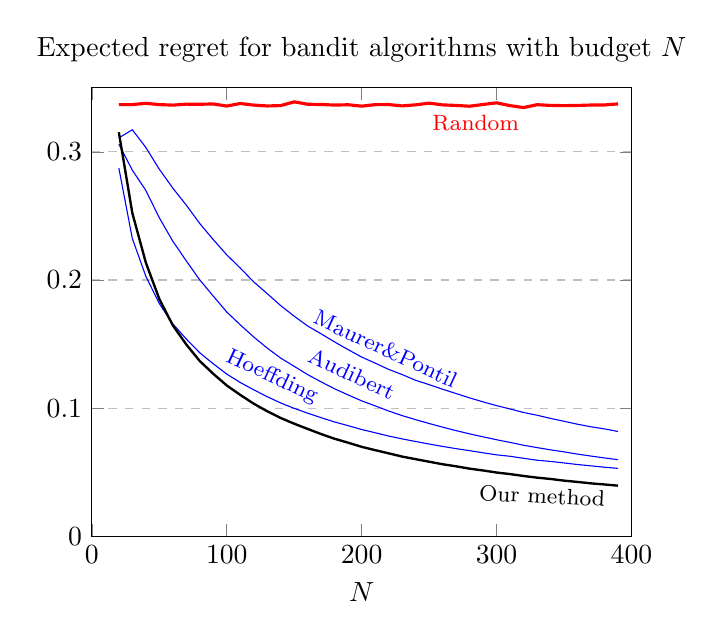
\begin{tikzpicture}
	\begin{axis}[
		title={Expected regret for bandit algorithms with budget $N$},
		xlabel={$N$},
		xmin=0, xmax=400,
		ymin=0, ymax=0.35,
		ymajorgrids=true,
		grid style=dashed
	]
	\addplot[blue] coordinates {
(20, 0.310951130364) (30, 0.317304721799) (40, 0.303506740539) (50, 0.286502047961) (60, 0.271750798627) (70, 0.258441105474) (80, 0.244084337607) (90, 0.23154222192) (100, 0.21962674765) (110, 0.209364293145) (120, 0.19849795256) (130, 0.189366124494) (140, 0.179985057504) (150, 0.17175192486) (160, 0.164084467112) (170, 0.15795328799) (180, 0.151595586119) (190, 0.145627208562) (200, 0.139841473843) (210, 0.135131674343) (220, 0.130210872033) (230, 0.126186563148) (240, 0.121707370459) (250, 0.118323364967) (260, 0.114727672756) (270, 0.11135242178) (280, 0.107973086348) (290, 0.104854372357) (300, 0.101926121277) (310, 0.0993107935735) (320, 0.0965791677494) (330, 0.0944273468526) (340, 0.0919468150041) (350, 0.0897017110445) (360, 0.0874165452919) (370, 0.085411858643) (380, 0.0837605537036) (390, 0.0817399520606)
		}node[pos=0.52](endofplotsquare){} ;
		\node [blue,above,rotate=-25] at (endofplotsquare) {\footnotesize Maurer\&Pontil};
	\addplot[red,line width=0.4mm] coordinates {
(20, 0.336942958587) (30, 0.336937645823) (40, 0.33793528862) (50, 0.336950104881) (60, 0.336542611243) (70, 0.337280819312) (80, 0.337200777509) (90, 0.337451863926) (100, 0.335809963856) (110, 0.337793875156) (120, 0.33654914298) (130, 0.335875820615) (140, 0.336188909491) (150, 0.339081235627) (160, 0.337206338081) (170, 0.337020887335) (180, 0.336563951732) (190, 0.336823591936) (200, 0.335728527085) (210, 0.336906574325) (220, 0.336981316156) (230, 0.33591692432) (240, 0.336764452534) (250, 0.338074323749) (260, 0.336715624161) (270, 0.336287747782) (280, 0.335670715253) (290, 0.337037990821) (300, 0.338315025894) (310, 0.336139218506) (320, 0.334622390817) (330, 0.336859134941) (340, 0.336317904597) (350, 0.336124307504) (360, 0.336277839902) (370, 0.336613274) (380, 0.336662753516) (390, 0.337483689505)
		}node[pos=0.715](endofplotsquare){} ;
		\node [red,below] at (endofplotsquare) {\footnotesize Random};
	\addplot[blue] coordinates {
(20, 0.28743290587) (30, 0.232382220095) (40, 0.20296927431) (50, 0.181606720226) (60, 0.165745102011) (70, 0.153907558509) (80, 0.143186137085) (90, 0.134590089348) (100, 0.126573002174) (110, 0.119992831407) (120, 0.11427869441) (130, 0.108890725408) (140, 0.104018433267) (150, 0.0998081258891) (160, 0.0960210094774) (170, 0.0924770288966) (180, 0.0891490256632) (190, 0.0862832212207) (200, 0.0832737235473) (210, 0.0807582587196) (220, 0.0781651915387) (230, 0.0759558632013) (240, 0.0739131187913) (250, 0.0719286269452) (260, 0.0700910030206) (270, 0.0683275770601) (280, 0.0667819025719) (290, 0.0650880008227) (300, 0.063500206177) (310, 0.0623834758598) (320, 0.0608073686435) (330, 0.0593185615513) (340, 0.0583541183652) (350, 0.0571870323598) (360, 0.0559368431009) (370, 0.054899877847) (380, 0.0538413306667) (390, 0.052941312716)
		}node[pos=0.29](endofplotsquare){} ;
		\node [blue,above,rotate=-25] at (endofplotsquare) {\footnotesize Hoeffding};
	\addplot[blue] coordinates {
(20, 0.306061843642) (30, 0.285754524727) (40, 0.269931278197) (50, 0.248615326378) (60, 0.230327866882) (70, 0.214922429349) (80, 0.200054374281) (90, 0.187439612189) (100, 0.175026770923) (110, 0.165017888537) (120, 0.155510023043) (130, 0.146850970099) (140, 0.139027366099) (150, 0.132617934825) (160, 0.126130658589) (170, 0.120431591885) (180, 0.115019877981) (190, 0.110269427886) (200, 0.105649535257) (210, 0.101741763249) (220, 0.0977283222415) (230, 0.0941251046786) (240, 0.0909714233319) (250, 0.0879807411491) (260, 0.0851390725522) (270, 0.0824012109451) (280, 0.079883684561) (290, 0.0775606819917) (300, 0.0752888280648) (310, 0.0732028631441) (320, 0.070993850246) (330, 0.069161594945) (340, 0.0673921094242) (350, 0.06583053422) (360, 0.0640749729154) (370, 0.0625422168091) (380, 0.0610836359114) (390, 0.0597357326982)
		}node[pos=0.35](endofplotsquare){} ;
		\node [blue,above right, rotate=-25] at (endofplotsquare) {\footnotesize Audibert};
	\addplot[line width=0.30mm] coordinates {
(20, 0.315351878837) (30, 0.252310598394) (40, 0.21365051234) (50, 0.185173245204) (60, 0.164633657836) (70, 0.149662482149) (80, 0.136725328307) (90, 0.126768907712) (100, 0.117664528623) (110, 0.110326598166) (120, 0.103415978409) (130, 0.0975188110085) (140, 0.0922740034531) (150, 0.0878113744221) (160, 0.0837255031) (170, 0.0797008178449) (180, 0.0760441489445) (190, 0.0729725631572) (200, 0.0697582108496) (210, 0.0671583991446) (220, 0.06468719194) (230, 0.0621409299865) (240, 0.0601285592881) (250, 0.0581341532097) (260, 0.0561603237441) (270, 0.0545519043883) (280, 0.0527161522742) (290, 0.0513002710141) (300, 0.0497036485461) (310, 0.0484855329667) (320, 0.0470042219926) (330, 0.045703669572) (340, 0.0446693501732) (350, 0.0433740760739) (360, 0.0423482852895) (370, 0.0412370883341) (380, 0.0403742986427) (390, 0.0394378538536)
		}node[pos=0.85](endofplotsquare){} ;
		\node [below,rotate=-3] at (endofplotsquare) {\footnotesize Our method};
	\end{axis}
	\end{tikzpicture}
	\vspace{-5pt}
	\caption{The expected regret of bandit algorithms and a baseline method in the example bandit problem: UCB method using our bound \eqref{eq:prob_bound}, Hoeffding's, Audibert et.al's, and Maurer \& Pontil's inequalities; and method of uniform randomly choosing an arm.}
	\label{biggraph44}
\end{figure}



The the performance of the four methods and the na\"{i}ve baseline are shown in Figure~\ref{biggraph44}.
From this figure, we see that minimizing an upper confidence bound utilizing our inequality \eqref{eq:prob_bound} results in best performance (lowest regret), except marginally in the region of very small sample budgets. 

It is somewhat surprising to see the more complicated EBB methods \cite{Maurer50empiricalbernstein,10.1007/978-3-540-75225-7_15} perform worse than the much simpler Hoeffding's inequality. As EBB inequalities are specifically constructed in a way to incorporate the estimate of the variance, then the potential advantage comes when there are sufficiently many samples for reliable variance estimation. However a bound without this construction (such as Hoeffding's inequality) may be tighter and more effective for small/medium sample budgets. 
As expected, the random method of choosing arms had a constant expected average regret across action budgets, as it does not learn with additional samples of the arms' rewards.


\section{Conclusion}\label{sec:conclusion}

In this paper, we have extended existing work on concentration inequalities to derive a new and stronger EBB.
Our EBB has many applications, in any setting where a mean value must be estimated with confidence, such as bandit problems.
Our EBB was shown to tighten known EBB-based confidence intervals by about a third, thereby improving the value of these types of concentration inequalities. 
This value was demonstrated in a MAB problem, where using our EBB in a UCB algorithm was shown to improve online learning performance.


\appendix
\section{Proofs}
\subsection{Small Proofs}\label{appendix:small}
%\small
\begin{proof}[Proof of Probability Union - Lemma \ref{prob_union}]
For any events $A$ and $B$\\
$\p(A\cup B) \le \p(A)+\p(B)$, hence for events $a>b$ and $b>c$:\\ $\p((a>b) \cup (b>c)) \le \p(a>b) + \p(b>c)$\\
If $a>c$, then $(a>b) \cup (b>c)$ is true irrespective of $b$, so:\\
$\p(a>c) \le \p((a>b) \cup (b>c))$
\hfill $\blacksquare$
\end{proof}

\begin{proof}[Proof of Variance Decomposition - Lemma \ref{variance1}]By expanding and $\hat{\sigma}^2$:\\
\(\quad\hat{\sigma}^2=\frac{1}{n-1}\sum_i\left(x_i-\frac{1}{n}\sum_jx_j \right)^2 
=\frac{1}{n-1}\left(\sum_ix_i^2-\frac{1}{n}\sum_{i,j}x_ix_j \right) = \frac{n}{n-1}\left(\hat{\sigma}_0^2-\hat{\mu}^2\right)\hfill\blacksquare\)
\end{proof}

\begin{proof}[Proof of Chernoff Bound - Lemma \ref{chernoff1}]\\
$\p(\hat{\mu}\ge t) =  \p\left(\exp\left(s\sum_{i=1}^nx_i\right)\ge \exp(snt)\right)$\\
\-\hspace{8mm}$\le \E\left[\exp\left(s\sum_{i=1}^nx_i\right)\right]\exp(-snt) \le \E\left[\exp\left(sX\right)\right]^n\exp(-snt)
$\\
using Markov's inequality and the i.i.d of the samples, respectively.
$\hfill\blacksquare$
\end{proof}



\subsection{A Proof of Bennett's inequality}\label{appendix:A}

\begin{theorem}[Parabola Fitting]\label{thm:parabola}
For $b>0$, $a<b$ and $z>0$, there exists an $\alpha,\beta,\gamma$ such that: $\alpha x^2+\beta x+\gamma\ge \exp(x)$ for all $a\le x\le b$, and:\\
\-\hspace{3mm}$z\alpha+\gamma = (z\exp(b) + b^2\exp(-z/b))(z + b^2)^{-1}$.
\end{theorem}
\begin{proof}
A example parabola $\alpha x^2+\beta x+\gamma$ which that satisfies these requirements tangentially touches the exponential curve at one point (at $x=f<b$) and intersects it at another (at $x=b$), as illustrated in Figure \ref{fig:graph1}.
Thus the parabola's intersection at $x=b$ and its tangential intersection at $x=f$ can be written in matrix algebra:
$$
\begin{bmatrix}
    \alpha \\
    \beta \\
	\gamma
\end{bmatrix}
=
\begin{bmatrix}
    b^2 & b & 1 \\
    f^2 & f & 1 \\
	2f  & 1 & 0
\end{bmatrix}^{-1}
\begin{bmatrix}
    \exp(b) \\
    \exp(f) \\
	\exp(f)
\end{bmatrix}$$
This gives our parabola parameters $\alpha,\beta,\gamma$, in terms of $f$ and $b$, hence:\\
\-\hspace{3mm}$z\alpha+\gamma = (((z+fb-b)(f-b-1)-b)e^f+(f^2+z)e^b)(b-f)^{-2}$\\
Minimizing with respect to $f$ occurs at $f=\frac{-z}{b}$ and gives the result.$\hfill\blacksquare$
\end{proof}

\begin{proof}[Proof of Bennett's inequlity -- Lemma \ref{hoeffdings1}]
As random variable X is bounded $a\le X\le b$, for any $s>0$, by Theorem \ref{thm:parabola}, there exist parameters $\alpha,\beta,\gamma$ such that, $\alpha s^2X^2+\beta sX+\gamma\ge \exp(sX)$ is always satisfied, hence for these we have:
\-\hspace{3mm}\(\E\left[\exp(sX)\right] \le \E[\alpha s^2X^2+\beta sX+\gamma] \le \alpha s^2\E[X^2]+\gamma \le \alpha  s^2\sigma^2+\gamma\)\\
\-\hspace{20.5mm}\( \le (\sigma^2\exp(sb) + b^2\exp(-s\sigma^2/b))(\sigma^2 + b^2)^{-1}\)\\
Hence by application of lemma \ref{chernoff1}:\\
\-\hspace{3mm}\(\p(\hat{\mu}\ge t) \;\le\; (\sigma^2\exp(sb) + b^2\exp(-s\sigma^2/b))^n((\sigma^2 + b^2)\exp(st))^{-n}\)\\
and finding the minimum with respect to $s$ completes the proof.$\hfill \blacksquare$
\end{proof}

\subsection{Remaining Proofs}\label{appendix:B}

\begin{proof}[Proof of Sample Square Bound - Lemma \ref{sample_squares}]
There exist parameters $\alpha,\gamma$ such for all $a\le X\le b$ that $\alpha X^2 + \gamma \ge \exp(-qX^2)$ whence:\\
\-\hspace{3mm}\(\E[\exp(-qX^2)] \le \E[\alpha x^2 +\gamma] \le \alpha\sigma^2 + \gamma \)\\
With $d=\max(b,-a)$, we choose (Fig \ref{fig:graph111}) $\alpha=(\exp(-qd^2)-1)d^{-2}$ and $\gamma=1$\\
Then applying lemma \ref{chernoff1} to the mean of the negated sample squares gives:\\
\-\hspace{3mm}\(
\p(-\hat{\sigma}_0^2\ge t) \le \left(\frac{\sigma^2}{d^2}\exp(-qd^2)+1-\frac{\sigma^2}{d^2}\right)^n\exp(-qnt) 
\)\\
Substituting $t$ for $y-\sigma^2$ and minimizing with $q$ completes the proof.
$\hfill\blacksquare$
\end{proof}

\begin{proof}[Proof of Sample Variance Bound - Lemma \ref{variance2}]
By Lemmas \ref{sample_squares} and \ref{variance1}:\\
\-\hspace{3mm}\(\p\left(\sigma^2 - \hat{\sigma}^2 > \frac{n}{n-1}\left(\hat{\mu}^2+y- \frac{1}{n}\sigma^2\right)\right) 
\le H_2^n\left(\frac{\sigma^2}{d^2},\frac{y}{d^2}\right)\)\\
Also, by manipulating the inner inequality of equation \ref{eq_no1}:\\ \-\hspace{3mm}\(\p\left(\frac{n}{n-1}\left(\hat{\mu}^2+y-\frac{1}{n}\sigma^2\right)\ge \frac{n}{n-1}\left(r^2+y-\frac{1}{n}\sigma^2\right)\right) \le H_1^n\left(\frac{\sigma^2}{b^2},\frac{r}{b}\right)+H_1^n\left(\frac{\sigma^2}{a^2},\frac{-r}{a}\right)\)\\
Applying lemma \ref{prob_union} to the above two equations gives:\\
\-\hspace{3mm}\(\p\left(\sigma^2 - \hat{\sigma}^2 > \frac{n}{n-1}\left(r^2+y-\frac{1}{n}\sigma^2\right)\right) \le H_2^n\left(\frac{\sigma^2}{d^2},\frac{y}{d^2}\right)+H_1^n\left(\frac{\sigma^2}{b^2},\frac{r}{b}\right)+H_1^n\left(\frac{\sigma^2}{a^2},\frac{-r}{a}\right)\)\\
For $w=\frac{n}{n-1}\left(r^2+y-\frac{1}{n}\sigma^2\right)$ there is a range of possible $r,y>0$ which we parameterise by value $\phi$, such that $0\le\phi\le 1$:\\
\-\hspace{3mm}\(y(\phi) = (1-\phi)\left(\frac{n-1}{n}w+\frac{1}{n}\sigma^2\right) \quad\text{and}\quad
r(\phi)^2 = \phi\left(\frac{n-1}{n}w+\frac{1}{n}\sigma^2\right)\)\\
Thus:\\
\-\hspace{3mm}\(\p\left(\sigma^2 - \hat{\sigma}^2 > w\right) 
\le H_2^n\left(\frac{\sigma^2}{d^2},\frac{y(\phi)}{d^2}\right) 
  + H_1^n\left(\frac{\sigma^2}{b^2},\frac{r(\phi)}{b}\right) + H_1^n\left(\frac{\sigma^2}{a^2},\frac{-r(\phi)}{a}\right)\)\\
The result of this proof follows by taking the minimum over $\phi$.
$\hfill\blacksquare$
\end{proof}





\begin{figure}%
\centering
\parbox{2in}{

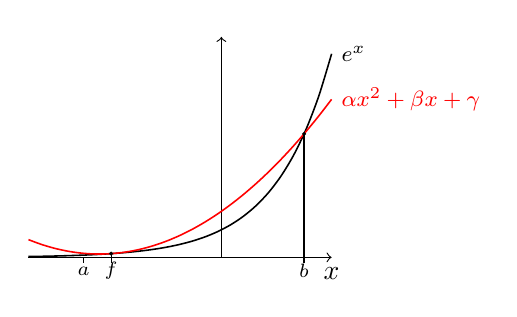
\begin{tikzpicture}[scale=0.7]
\draw[->] (-3.5,0) -- (2,0) node[anchor=north] {$x$};
\draw[->] (0,0) -- (0,4) node[anchor=east] {};
\draw[smooth, domain=-3.5:2.0, color=black, line width=0.20mm] 
    plot (\x,{e^(\x)/2}) node [right] {\footnotesize $e^x$};
\draw[smooth, domain=-3.5:2.0, color=red, line width=0.20mm] 
    plot (\x,{(0.316137167001903*\x*\x + 1.39988395124422*\x + 1.67055451771745)/2}) node [right] {\footnotesize $\alpha x^2+\beta x+\gamma$};
\draw (1.5,-0.1) -- (1.5,{e^(1.5)/2});
\draw (-2,-0.1) -- (-2,{e^(-2)/2});
\draw (-2.5,-0.1) -- (-2.5,0);
\draw[black,fill] (1.5,{e^(1.5)/2}) circle (0.25mm);
\draw[black,fill] (-2,{e^(-2)/2}) circle (0.25mm);
\draw	(-2.5,-0.25) node{{\scriptsize $a$}}
		(-2,-0.25) node{{\scriptsize $f$}}
		(1.5,-0.25) node{{\scriptsize $b$}};
\end{tikzpicture}

\caption{A parabola parametarised by touching and intercepting points $f,b$ above an exponential curve for all $a\le x\le b$}%
\label{fig:graph1}}%
\qquad
\begin{minipage}{2in}%

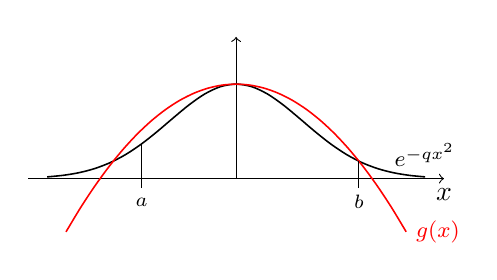
\begin{tikzpicture}[scale=1.2]
\draw[->] (-2.2,0) -- (2.2,0) node[anchor=north] {$x$};
\draw[->] (0,0) -- (0,1.5) node[anchor=east] {};
\draw[smooth, domain=-2.0:2.0, color=black, line width=0.20mm] 
    plot (\x,{e^(-(\x*\x))}) node [above] {\footnotesize $e^{-qx^2}$};
\draw[smooth, domain=-1.8:1.8, color=red, line width=0.20mm] 
    plot (\x,{-0.4825*\x*\x+1}) node [right] {\footnotesize $g(x)$};
\draw (1.3,-0.1) -- (1.3,{e^(-1.3*1.3)});
\draw (-1,-0.1) -- (-1,{e^(-1*1)});
\draw	(-1,-0.25) node{{\scriptsize $a$}}
		(1.3,-0.25) node{{\scriptsize $b$}};
\end{tikzpicture}

\caption{$g(x)=(e^{-qd^2}-1)d^{-2}x^2+1$ over function $f(x)=e^{-qx^2}$ for all $a\le x\le b$ where $d=\max(b,-a)$; in the case $a=-1,b=1.3,q=1$}%
\label{fig:graph111}%
\end{minipage}%
\end{figure}





%\bibliographystyle{splncs04}
%\bibliography{references}

\begin{thebibliography}{10}
\providecommand{\url}[1]{\texttt{#1}}
\providecommand{\urlprefix}{URL }
\providecommand{\doi}[1]{https://doi.org/#1}

\bibitem{AgarwalDekelXiao2010}
Agarwal, A., Dekel, O., Xiao, L.: Optimal algorithms for online convex
  optimization with multi-point bandit feedback. In: 23rd Annual Conf. Learning
  Theory (COLT'10) (2010)

\bibitem{Aggarwal2015}
Aggarwal, C.C.: Data Mining: The Textbook, chap. Outlier analysis, pp.
  237--263. Springer Publishing Company, Incorporated (2015)

\bibitem{AudibertBubeck_COLT2009}
Audibert, J.Y., Bubeck, S.: Minimax policies for adversarial and stochastic
  bandits. In: 22nd Annual Conf. Learning Theory (COLT'09) (2009)

\bibitem{10.1007/978-3-540-75225-7_15}
Audibert, J.Y., Munos, R., Szepesv{\'a}ri, C.: Tuning bandit algorithms in
  stochastic environments. In: Hutter, M., Servedio, R.A., Takimoto, E. (eds.)
  Algorithmic Learning Theory. pp. 150--165. Springer Berlin Heidelberg,
  Berlin, Heidelberg (2007)

\bibitem{AuerCesa-BianchiEtal_SIAM2003}
Auer, P., Cesa-{B}ianchi, N., Freund, Y., Schapire, R.: The
  non-stochasticmulti-armed bandit problem. SIAM Journal on Computing
  \textbf{31}(1),  48--77 (2003)

\bibitem{Auer2002}
Auer, P., Cesa-Bianchi, N., Fischer, P.: Finite-time analysis of the multiarmed
  bandit problem. Machine Learning  \textbf{47}(2),  235--256 (May 2002)

\bibitem{10.2307/2282438}
Bennett, G.: Probability inequalities for the sum of independent random
  variables. Journal of the American Statistical Association  \textbf{57}(297),
   33--45 (1962)

\bibitem{Bentkus08boundsfor}
Bentkus, V., Ju\v{s}kevi\v{c}ius, T.: Bounds for tail probabilities of
  martingales using skewness and kurtosis. Lithuanian Mathematical Journal
  \textbf{48}(1),  30--37 (Jan 2008)

\bibitem{MR3363542}
Bercu, B., Delyon, B., Rio, E.: Concentration inequalities for sums and
  martingales. Springer Briefs in Mathematics, Springer (2015)

\bibitem{Burnstein1}
Bernstein, S.N.: On a modification of {C}hebyshev’s inequality and of the
  error formula of {L}aplace. Uchenye Zapiski Nauch.-Issled. Kaf. Ukraine,
  Sect. Math  \textbf{1},  38--48 (1924)

\bibitem{8000571}
Bhaduri, M., Zhan, J., Chiu, C., Zhan, F.: A novel online and non-parametric
  approach for drift detection in big data. IEEE Access  \textbf{5},
  15883--15892 (2017)

\bibitem{Chebyshev1}
Bienaymé, I.J.: Considérations àl'appui de la découverte de {L}aplace.
  Comptes Rendus de l'Académie des Sciences  \textbf{37},  309--324 (1853)

\bibitem{Boucheron2004}
Boucheron, S., Lugosi, G., Bousquet, O.: Concentration inequalities. In:
  Bousquet, O., von Luxburg, U., R{\"a}tsch, G. (eds.) Advanced Lectures on
  Machine Learning: ML Summer Schools 2003, Canberra, Australia, February 2 -
  14, 2003, T{\"u}bingen, Germany, August 4 - 16, 2003, Revised Lectures, pp.
  208--240. Springer Berlin Heidelberg, Berlin, Heidelberg (2004)

\bibitem{Boucheron_concentrationinequalities}
Boucheron, S., Lugosi, G., Massart, P.: Concentration inequalities using the
  entropy method. The Annals of Probability  \textbf{31}(3),  1583--1614 (2003)

\bibitem{Cesa-BianchiLugosi2006}
Cesa-{B}ianchi, N., Lugosi, G.: Prediction, Learning, and Games. Cambridge
  University Press (2006)

\bibitem{efron1981}
Efron, B., Stein, C.: The jackknife estimate of variance. Annals of Statistics
  \textbf{9}(3),  586--596 (05 1981)

\bibitem{FlaxmanKalaiMcMahan2005}
Flaxman, A., Kalai, A., McMahan, B.: Online convex optimization in the bandit
  setting: Gradient descent without a gradient. In: Proc. 16th Annual ACM-SIAM
  Symposium on Discrete Algorithms (SODA'05). p. 385–394 (2005)

\bibitem{hoeffding1}
Hoeffding, W.: Probability inequalities for sums of bounded random variables.
  Journal of the American Statistical Association  \textbf{58}(301),  13--30
  (Mar 1963)

\bibitem{KiferShaiGehrke2004}
Kifer, D., Ben-David, S., Gehrke, J.: Detecting change in data streams. In:
  Proc. 30th Int. Conf. Very Large Data Bases (VLDB'04). pp. 180--191. VLDB '04
  (2004)

\bibitem{Lai_1985}
Lai, T., Robbins, H.: Asymptotically efficient adaptive allocation rules.
  Advances in Applied Mathematics  \textbf{6}(1),  4--22 (Mar 1985)

\bibitem{MR2245497}
Maurer, A.: Concentration inequalities for functions of independent variables.
  Random Structures \& Algorithms  \textbf{29}(2),  121--138 (2006)

\bibitem{Maurer50empiricalbernstein}
Maurer, A., Pontil, M.: Empirical {B}ernstein bounds and sample variance
  penalization. stat. Proceedings of the 22nd Annual Conf. Learning Theory
  (COLT'09) (June 2009)

\bibitem{Mnih:2008:EBS:1390156.1390241}
Mnih, V., Szepesv\'{a}ri, C., Audibert, J.Y.: Empirical {B}ernstein stopping.
  In: Proc. 25th Int. Conf. Machine Learning (ICML'08). pp. 672--679 (2008)

\bibitem{Pinelis2014}
Pinelis, I.: On the {B}ennett-{H}oeffding inequality. Annales de i'Institut
  Henri Poincar\'{e} - Probabilit\'{e}s et Statistiques  \textbf{50}(1),
  15--27 (2014)

\bibitem{Zia-UrRehman2012}
Rehman, M.Z., Li, T., Li, T.: Exploiting empirical variance for data stream
  classification. Journal of Shanghai Jiaotong University (Science)
  \textbf{17}(2),  245--250 (Apr 2012)

\bibitem{Robbins1952}
Robbins, H.: Some aspects of the sequential design of experiments. Bulletin of
  the AMS  \textbf{55},  527--535 (1952)

\bibitem{zbMATH05780164}
Sharma, R., Gupta, M., Kapoor, G.: Some better bounds on the variance with
  applications. Journal of Mathematical Inequalities  \textbf{4}(3),  355--363
  (2010)

\bibitem{Talagrand1995}
Talagrand, M.: Concentration of measure and isoperimetric inequalities in
  product spaces. Publications Math{\'e}matiques de l'Institut des Hautes
  {\'E}tudes Scientifiques  \textbf{81}(1),  73--205 (Dec 1995)

\bibitem{zbMATH00812598}
Talagrand, M.: The missing factor in {H}oeffding's inequalities. Annales de
  l'Institut Henri Poincare, Probability and Statistics  \textbf{31}(4),
  689--702 (1995)

\bibitem{DBLP:conf/aaai/ThomasTG15}
Thomas, P.S., Theocharous, G., Ghavamzadeh, M.: High-confidence off-policy
  evaluation. In: Proc. 29th AAAI Conf. Artificial Intelligence (AAAI'15). pp.
  3000--3006 (2015)

\bibitem{Tran-ThanhChapmanRJ_AAAI2009}
Tran-Thanh, L., Chapman, A.C., Rogers, A., Jennings, N.R.: Knapsack based
  optimal policies for budget-limited multi-armed bandits. In: Proc.~26th AAAI
  Conf. Artificial Intelligence (AAAI'12). pp. 1134--1140. AAAI'12 (2012)

\end{thebibliography}



\end{document}


